\documentclass[a4paper, 12pt]{article}
\usepackage[T1]{fontenc}
\usepackage{lmodern}
\usepackage{color}
\usepackage{amsfonts}
\usepackage{epstopdf}
\usepackage{matlab}
\usepackage{booktabs}
%\documentclass{book}
\usepackage{blindtext}
\usepackage{hyperref}
\usepackage[brazil]{babel}
\usepackage{amssymb}
\usepackage[utf8]{inputenc}
\usepackage{amsmath}
\usepackage{indentfirst}
\usepackage{graphicx}
\usepackage{listings}
\usepackage{tcolorbox}
\usepackage{upgreek}
\usepackage{multicol,lipsum}
\usepackage[a4paper,
top=3cm, left=3cm, bottom=3cm, right=3cm]{geometry}
\usepackage{setspace}
\usepackage{multirow}
\usepackage{float}
\usepackage[dvipsnames]{xcolor}
\usepackage[table]{xcolor}
%\usepackage{pdflscape}
\usepackage[DIV=15]{typearea}
\usepackage[nottoc]{tocbibind}
\usepackage[sort,numbers]{natbib}
%\usepackage{cite}
\usepackage{matlab}

\usepackage[utf8]{inputenc}
\usepackage[T1]{fontenc}
\usepackage{lmodern}
\usepackage{graphicx}
\usepackage{color}
\usepackage{hyperref}
\usepackage{amsmath}
\usepackage{amsfonts}
\usepackage{epstopdf}
\usepackage[table]{xcolor}
\usepackage{matlab}


\documentclass[letterpaper]{article}
% bib pack %%%%%%%%%%%%%%%%%%%%%%%%%%%%%%%%%%%%%%%%%%%%%%%%%%%%%%%%%%%%%%%%%%%%%
\usepackage[utf8]{inputenc}
\usepackage{geometry}
    \geometry{left=3cm,right=2cm,top=2cm,bottom=2cm}
%
\usepackage[spanish]{babel}
%
\usepackage[fixlanguage]{babelbib}
    \bibliographystyle{babunsrt}
%
\usepackage{url}

\begin{document}
%\maketitle

\begin{titlepage}
	\begin{center}
		

\vspace{10pt}
%\begin{figure}[H][!ht]
%\centering
%
\includegraphics{puc-rio-logo.png}

%\end{figure}
\begin{figure}[!ht]
\centering

\includegraphics{images/puc-rio-logo.png}
\end{figure}
\huge{Instrumentação Eletrônica}
        \vspace{70pt}
        
		\textbf{ENG1027}
		\textbf{\large{\\ }}
		
		\vspace{30pt}
		\textbf{\small{\\Atividade 03 - Aula Prática de Simulação de Circuitos com Diodos}}
		\vspace{75pt}
		
	\end{center}
	
	\begin{flushleft}
		\begin{tabbing}
			Alunos\qquad\qquad\=\>Paloma Sette - 1621595\\
			\>Leonardo Matias - 1721693 \\
			Professor\>Igor Braga de Paula\\
	\end{tabbing}
		  
	\end{flushleft}
	\begin{center}
		%\vspace{\fill}
		\vspace{215pt}
		Rio de Janeiro, 28 de Maio de 2023
	\end{center}
\end{titlepage}
%%%%%%%%%%%%%%%%%%%%%%%%%%%%%%%%%%%%%%%%%%%%%%%%%%%%%%%%%%%



\newpage
\pagenumbering{arabic}

\newpage

%\newcommand{\listequationsname}{Lista de Equações}
%\newlistof{myequations}{equ}{\listequationsname}
%\newcommand{\myequations}[1]{%
%\addcontentsline{equ}{myequations}{\protect\numberline{\theequation}#1}\par}

%\listofmyequations
%%%%%%%%%%%%%%%%%%%%%%%%%%%%%%%%%%%%%%%%%%%%%%%%%%%%%%%%%%%
\newpage
\tableofcontents
\thispagestyle{empty}

\newpage
\pagenumbering{arabic}

\newpage

%\newcommand{\listequationsname}{Lista de Equações}
%\newlistof{myequations}{equ}{\listequationsname}
%\newcommand{\myequations}[1]{%
%\addcontentsline{equ}{myequations}{\protect\numberline{\theequation}#1}\par}

%\listofmyequations
\newpage


\newpage

\listoffigures
\thispagestyle{empty}

\newpage
%%%%%%%%%%%%%%%%%%%%%%%%%%%%%%%%%%%%%%%%%%%%%%%%%%%%%%%%%
%%%%%%%%%%%%%%%%%%%%%%%%%%%%%%%%%%%%%%%%%%%%%%%%%%%

\newpage

\thispagestyle{empty}

\newpage


\section{Introdução}
Este relatório refere-se à terceira sequência de atividades da disciplina de Instrumentação Eletrônica (ENG1027) de 2023.1. \\

Descreveremos os resultados ocorridos nos experimentos de simulação de circuitos com diodos.\\

Utilizamos dois softwares de simulação. Para o retificador simples (com somente 1 diodo) e um resistor, utilizamos o LTSpice. Para as demais simulações, foi utilizado o TopSpice.


\section{ Retificador Simples}

A curva relacionada à tensão da fonte está em azul escuro e, embora esteja com pouco contraste, é possível visualizar bem aproximando um pouco na tela. \\

Podemos observar as diferenças nas curvas com base nas alterações dos valores das capacitâncias. \\

Para o primeiro, temos um tempo de assentamento  de $\tau = RC = 1k\Omega*10^{-7} = 10^{-4}s $
\begin{figure}[H]
\centering
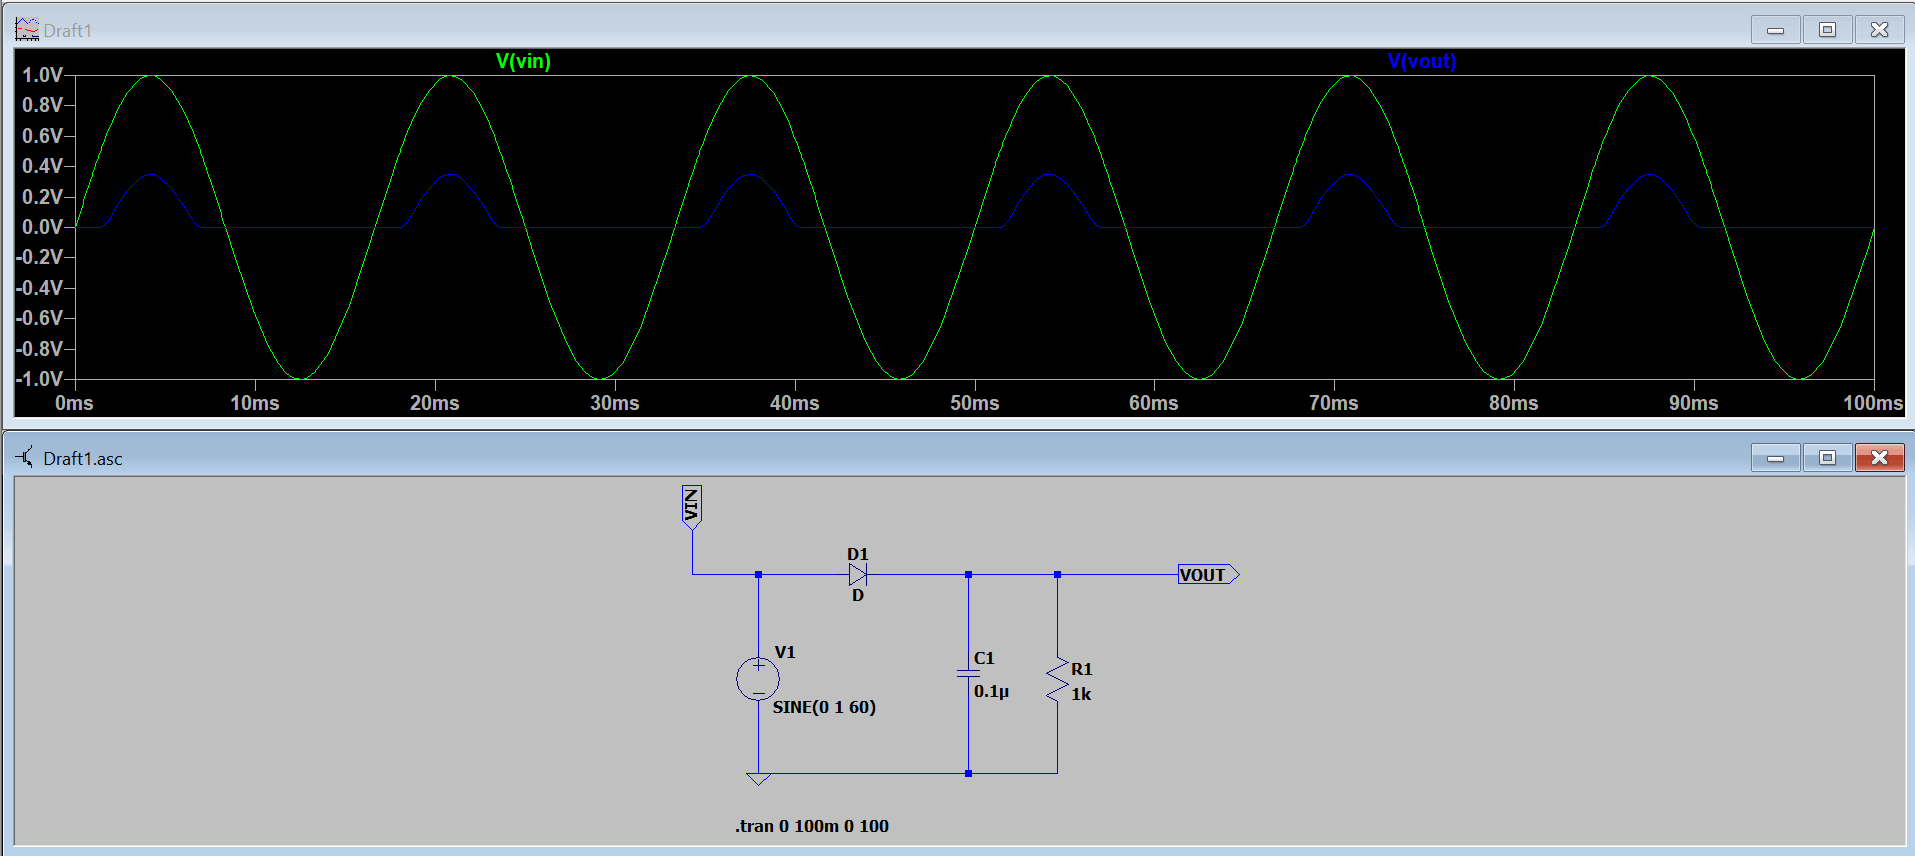
\includegraphics[scale = 0.45]{images/simulacao1.1.png}
\label{filtro1}
\caption{LTSpice: Retificador simples com C = 0.1uF}
\end{figure}

Para o segundo, temos um tempo de assentamento  de $\tau = RC = 1k\Omega*100\mu F = 0.1s $

\begin{figure}[H]
\centering
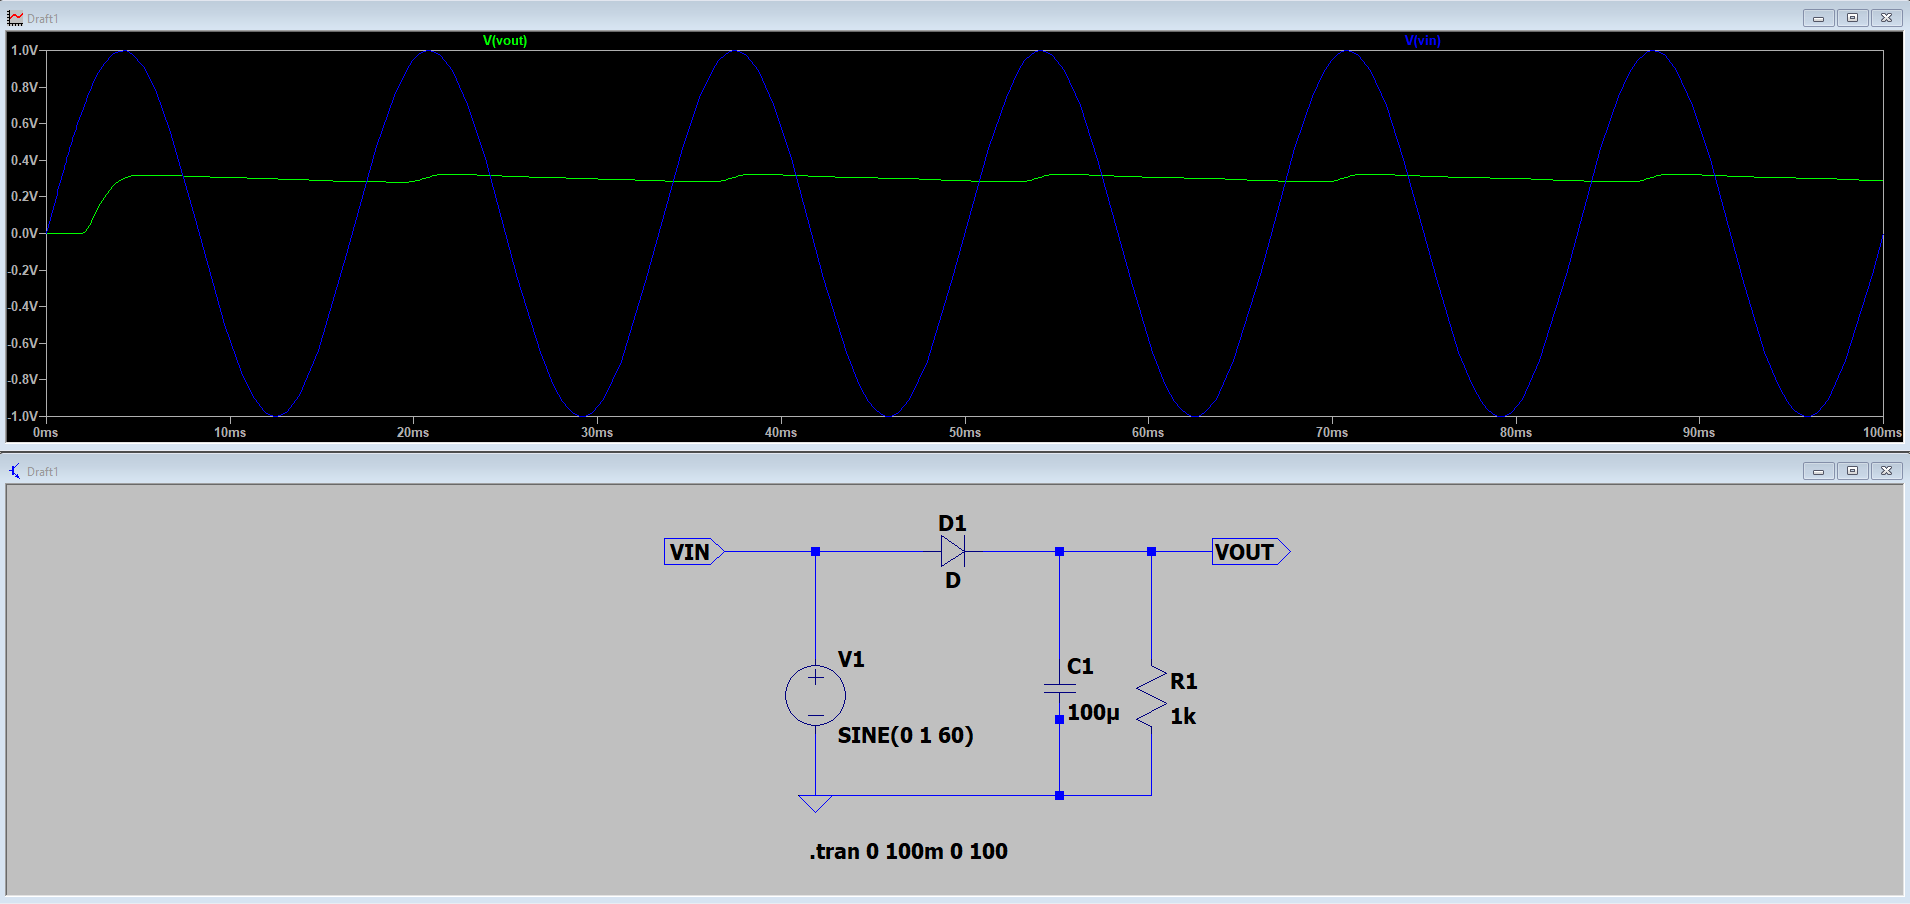
\includegraphics[scale = 0.31]{images/simulacao1.2.png}
\label{filtro1}
\caption{LTSpice: Retificador simples com C = 100uF}
\end{figure}

Para o terceiro, temos um tempo de assentamento  de $\tau = RC = 1k\Omega*0.015\mu F = 1.5 * 10^{-5}s $
\begin{figure}[H]
\centering
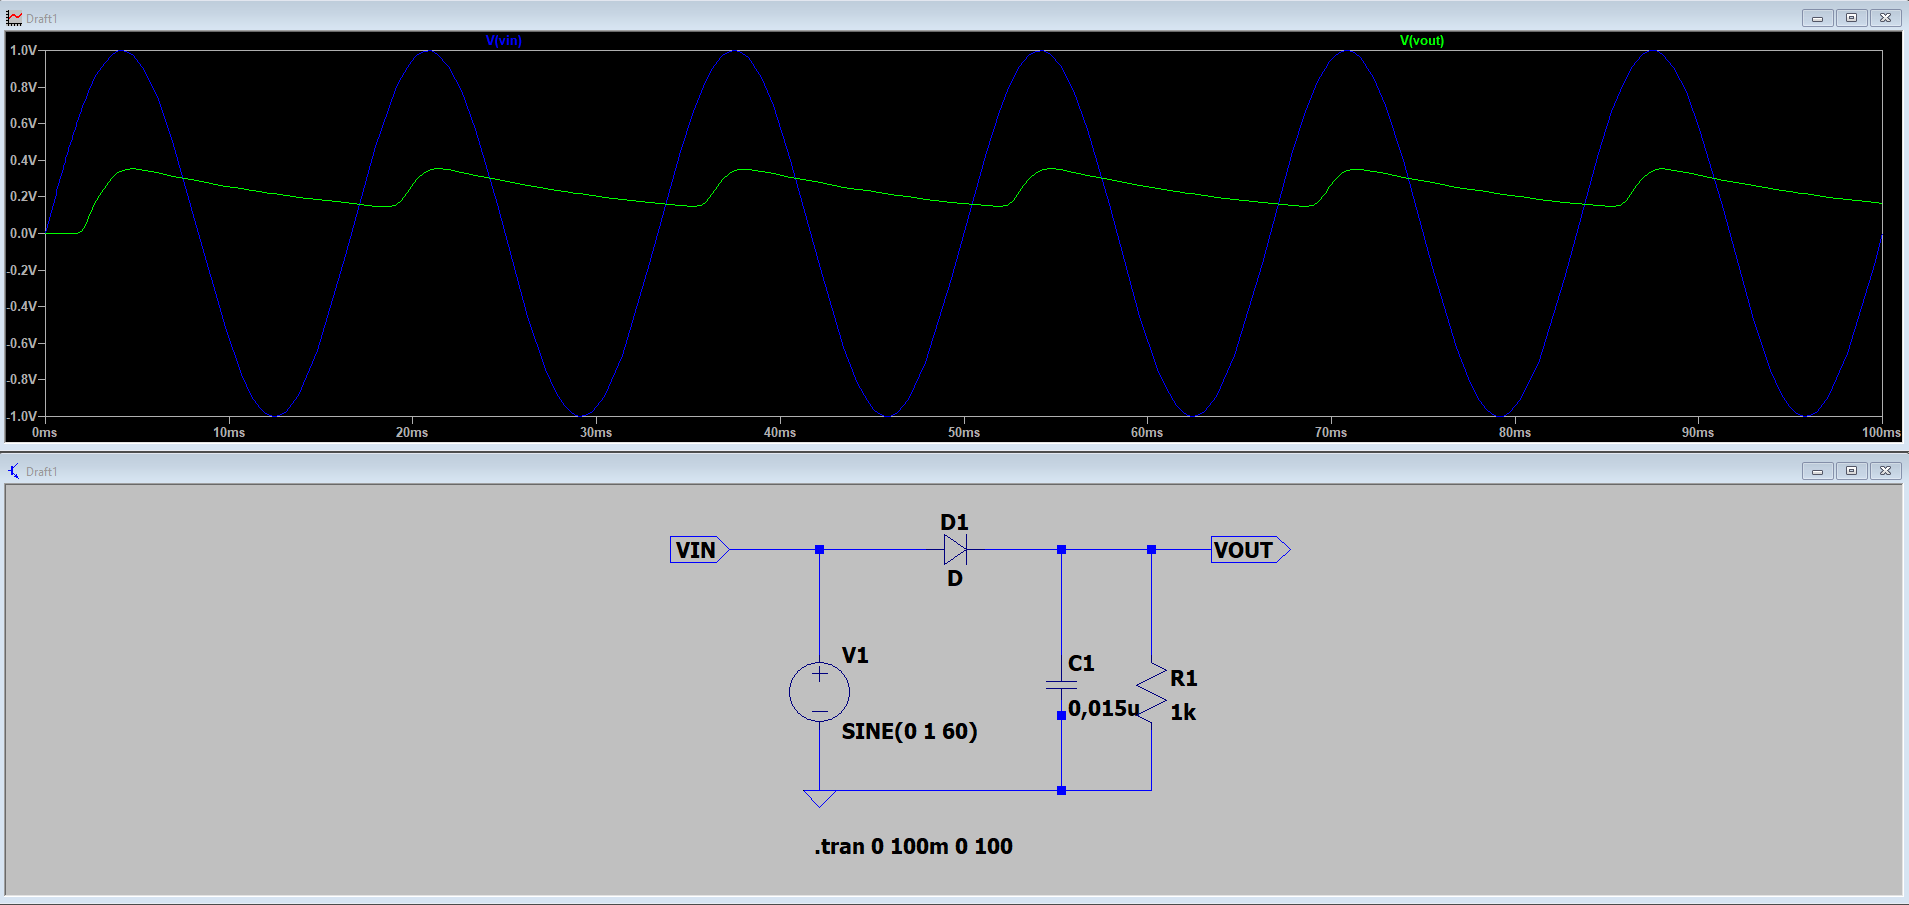
\includegraphics[scale = 0.31]{images/simulacao1.3.png}
\label{filtro1}
\caption{LTSpice: Retificador simples com C = 0.015uF}
\end{figure}

\section{Filtragem com a Ponte Retificadora}
\subsection{Ponte + Resistor}

\begin{figure}[H]
\centering
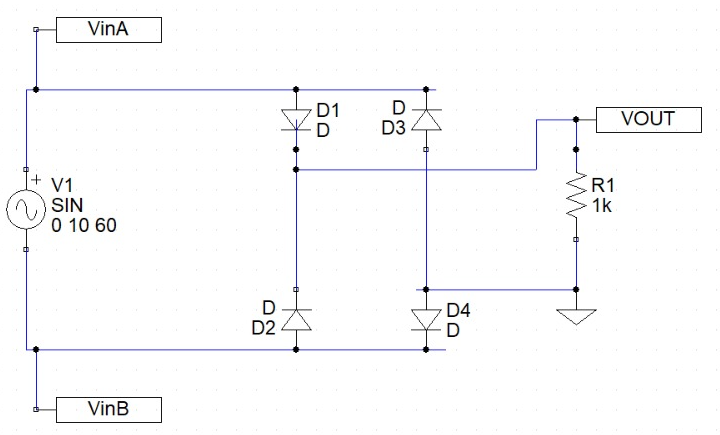
\includegraphics[scale = 0.48]{images/simulacao2.1.png}
\label{filtro1}
\caption{TopSpice: Circuito com a ponte + resistor}
\end{figure}

A simulação é de um circuito retificador de onda completa, que converte uma tensão AC em uma tensão DC mais suave.

O gráfico mostra duas formas de onda, uma de entrada (V(VINA)-V(VINB)) e outra de saída (V(VOUT)). A forma de onda de entrada é a diferença de potencial entre VINA e VINB.

A forma de onda de saída (V(VOUT)) mostra a tensão DC nos circuitos retificadores e de filtragem. A forma de onda mostra um aumento gradual na tensão à medida que o capacitor de filtragem armazena energia durante os picos positivos de tensão, e depois libera essa energia quando a tensão cai abaixo do nível de pico.



\begin{figure}[H]
\centering
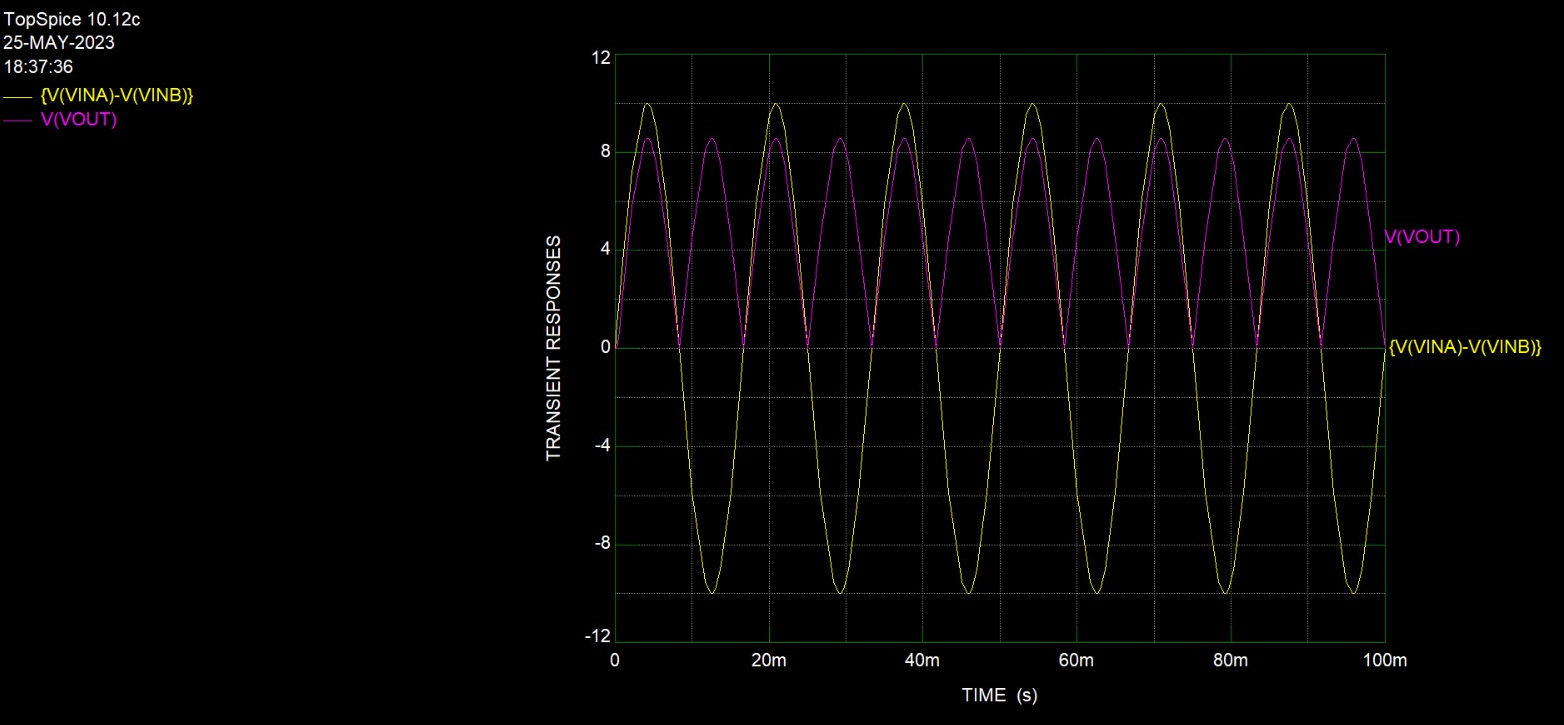
\includegraphics[scale = 0.4]{images/simulacao2.1_g.png}
\label{filtro1}
\caption{TopSpice: Gráfico - Circuito com a ponte + resistor}
\end{figure}


\subsection{Ponte + Capacitor + Resistor}

Este circuito consiste em uma ponte retificadora, com um capacitor de 100uF e um resistor de 1k conectados em paralelo entre a saída da ponte retificadora e o terra. A entrada é composta por duas fontes de tensão: V1, que gera um sinal senoidal de 10V e frequência de 60Hz para a entrada VinA, e VinB, que é conectada ao ponto central da ponte.\\

Os diodos D1, D3 e D4 estão posicionados para conduzir apenas durante o semiciclo positivo da onda de entrada, enquanto D2, D4 e D5 conduzem apenas no semiciclo negativo. Isso faz com que o sinal de saída seja uma aproximação do valor absoluto da entrada, com o potencial de VinB funcionando como referência de terra.\\

O capacitor de 100uF e o resistor de 1k formam um filtro passa-baixa que suaviza o sinal retificado e atua como uma carga de saída para a ponte retificadora, evitando que a tensão de saída flutue sem carga.\\

\subsubsection{C = 0.1uF}

\begin{figure}[H]
\centering
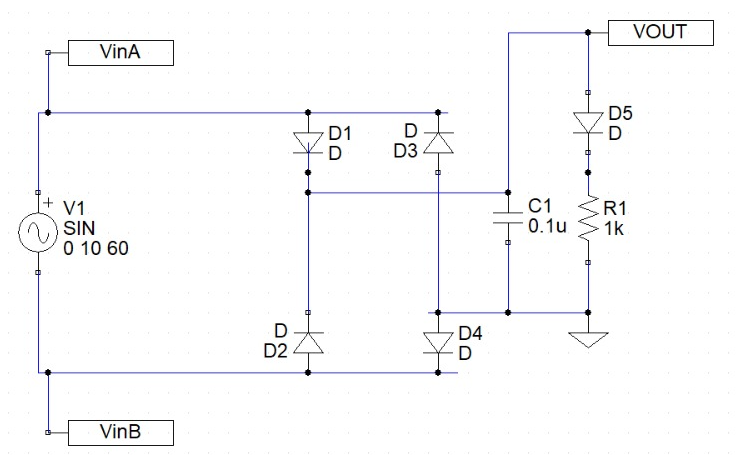
\includegraphics[scale = 0.48]{images/simulacao3.1_0.1u.png}
\label{filtro1}
\caption{TopSpice: Circuito com a ponte + capacitor = 0.1uF + resistor}
\end{figure}

\begin{figure}[H]
\centering
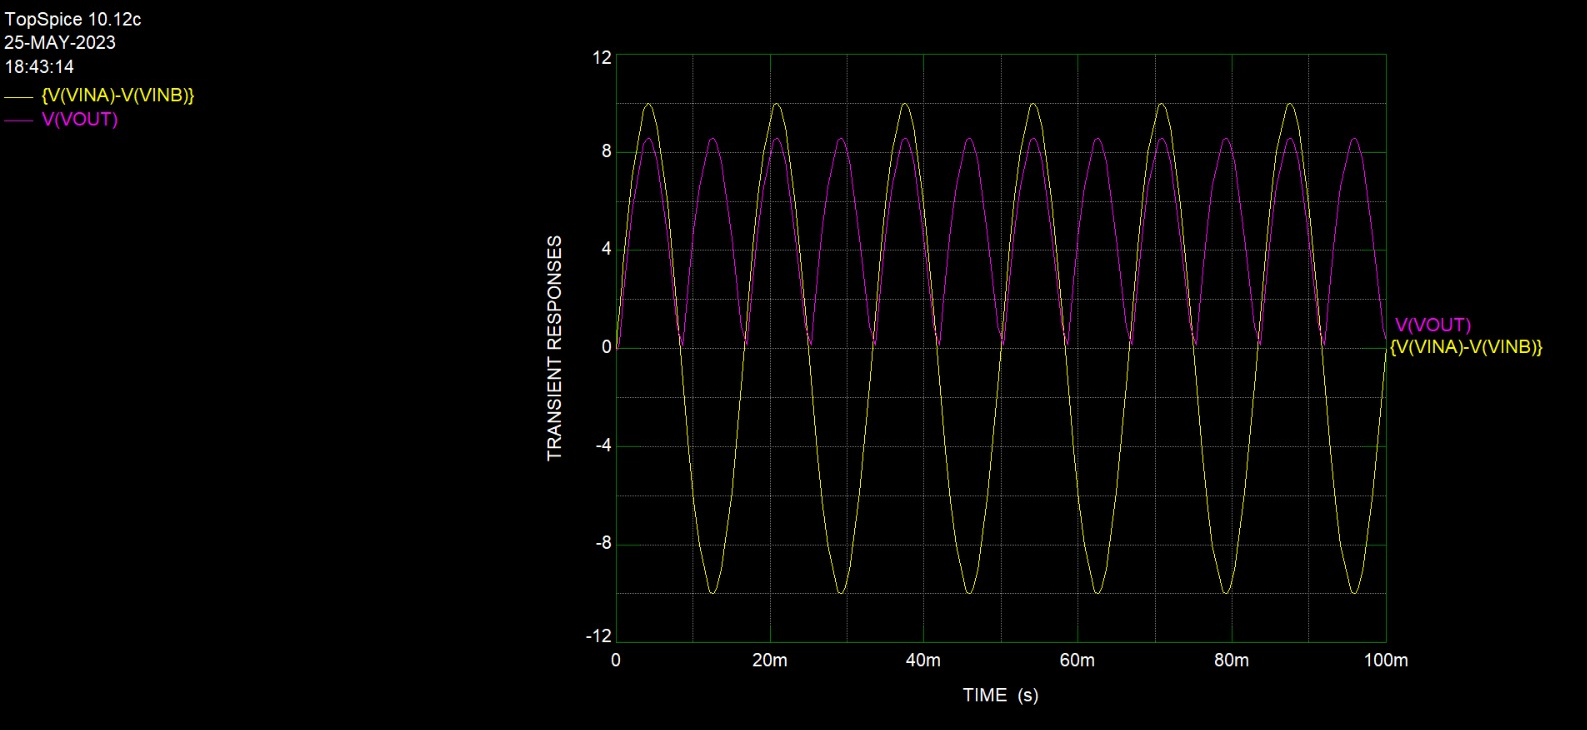
\includegraphics[scale = 0.4]{images/simulacao3.1_0.1ug.png}
\label{filtro1}
\caption{TopSpice: Gráfico - Circuito com a ponte + capacitor = 0.1uF + resistor}
\end{figure}


\subsubsection{C = 100uF}
Aumentar o valor do capacitor para $100\mu F$ aumenta o tempo de carga do circuito, o que resulta em um comportamento transitório mais lento e uma resposta de saída mais suave. O capacitor funciona como um reservatório de carga e tem a função de suavizar a tensão de saída ao agir como um filtro passa-baixas.\\

Em outras palavras, o aumento do valor do capacitor permite que mais carga seja armazenada em um determinado período de tempo, o que resulta em uma tensão de saída mais estável e menos sujeita a flutuações. Essa mudança no tamanho do capacitor pode estar afetando a "constante de tempo" do filtro passa-baixas, que determina a frequência de corte ou a taxa de mudança da tensão de saída.


\begin{figure}[H]
\centering
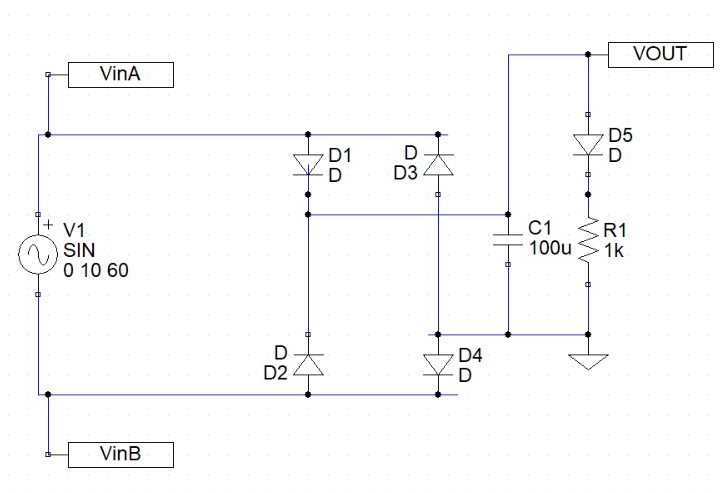
\includegraphics[scale = 0.48]{images/simulacao3.2_100u.png}
\label{filtro1}
\caption{TopSpice: Circuito com a ponte + capacitor=100uF + resistor}
\end{figure}

\begin{figure}[H]
\centering
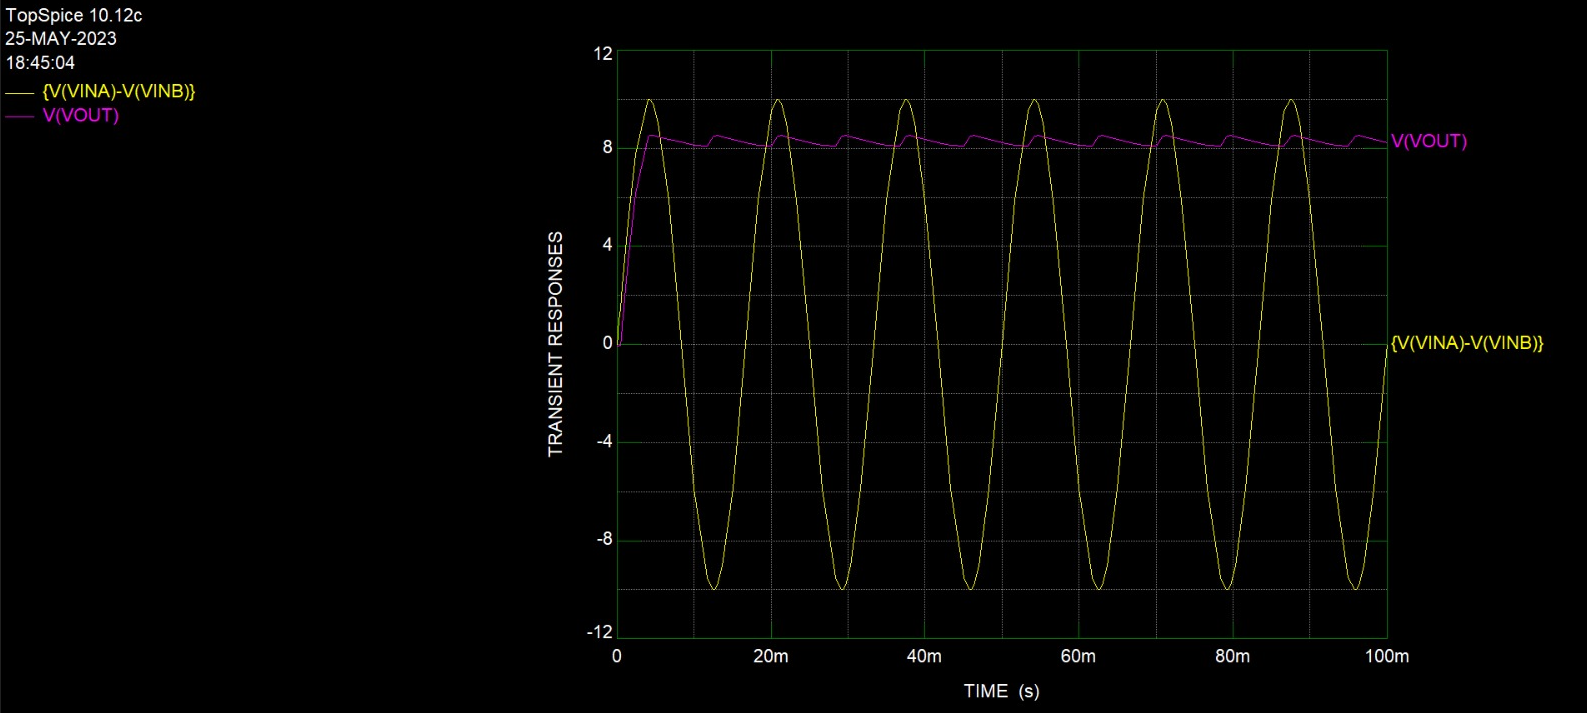
\includegraphics[scale = 0.4]{images/simulacao3.2_100ug.png}
\label{filtro1}
\caption{TopSpice: Gráfico - Circuito com a ponte + capacitor=100uF + resistor}
\end{figure}

\subsubsection{C = 0.015uF}
Ao diminuir o valor do capacitor para $0.015\mu F$, a frequência de corte do filtro passa-baixo diminui. Isso significa que o filtro permitirá uma passagem de frequência mais alta do que para o capacitor de $0.1\mu F$, mas ainda atenuará sinais com frequências mais altas do que o novo valor de frequência de corte.\\

O resultado disso pode ser um aumento de oscilações na saída, pois menos sinais de alta frequência estarão sendo filtrados pelo capacitor. O comportamento transitório do circuito também pode ser mais rápido do que para o capacitor de $100\mu F$, devido ao tempo de carga mais curto.

\begin{figure}[H]
\centering
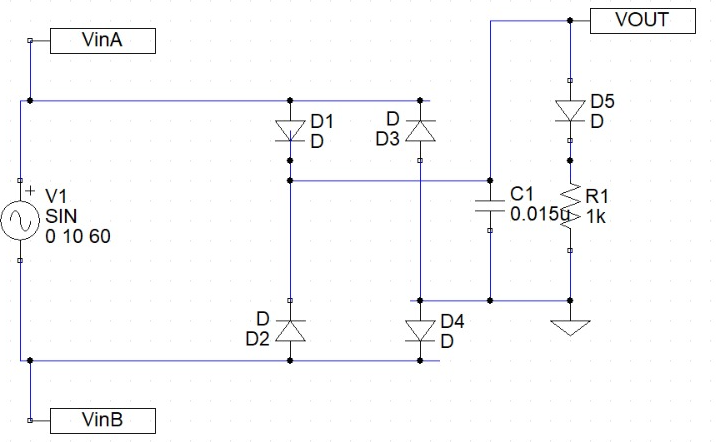
\includegraphics[scale = 0.48]{images/simulacao3.3_0.015u.png}
\label{filtro1}
\caption{TopSpice: Circuito com a ponte + capacitor=0.015uF + resistor}
\end{figure}

\begin{figure}[H]
\centering
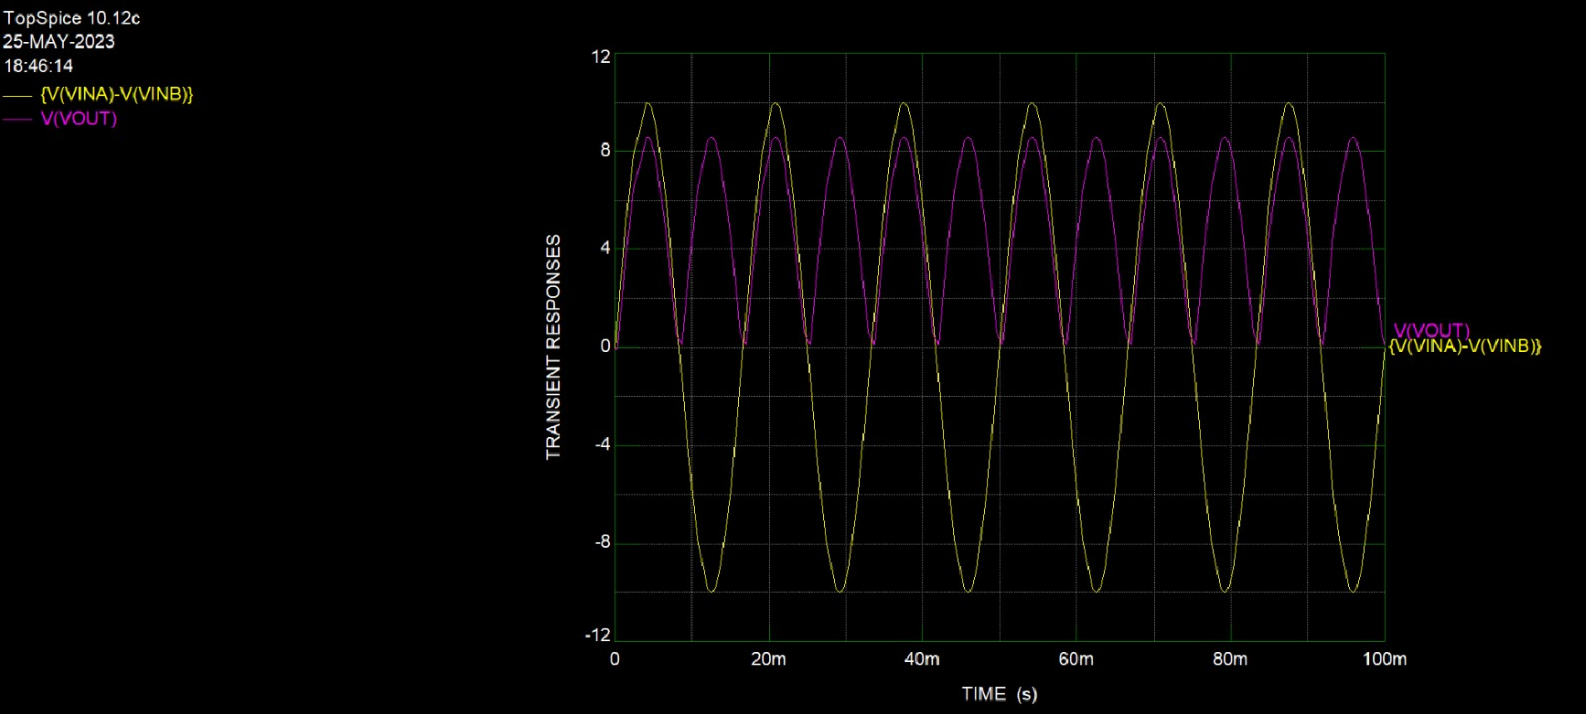
\includegraphics[scale = 0.4]{images/simulacao3.3_0.015ug.png}
\label{filtro1}
\caption{TopSpice: Gráfico - Circuito com a ponte + capacitor=0.015uF + resistor}
\end{figure}


\newpage
% REFERENCIAS %%%%%%%%%%%%%%%%%%%%%%%%%%%%%%%%%%%%%%%%%%%%%%%%%%%%%%%%%%%%%%


\end{document}